\documentclass[a4paper,11pt]{article}

\usepackage[spanish]{babel}
\usepackage{graphicx}
\usepackage[ansinew]{inputenc}
\usepackage[utf8]{inputenx}

\title{\textbf{Trabajo Práctico Aéreos} \\[1cm] 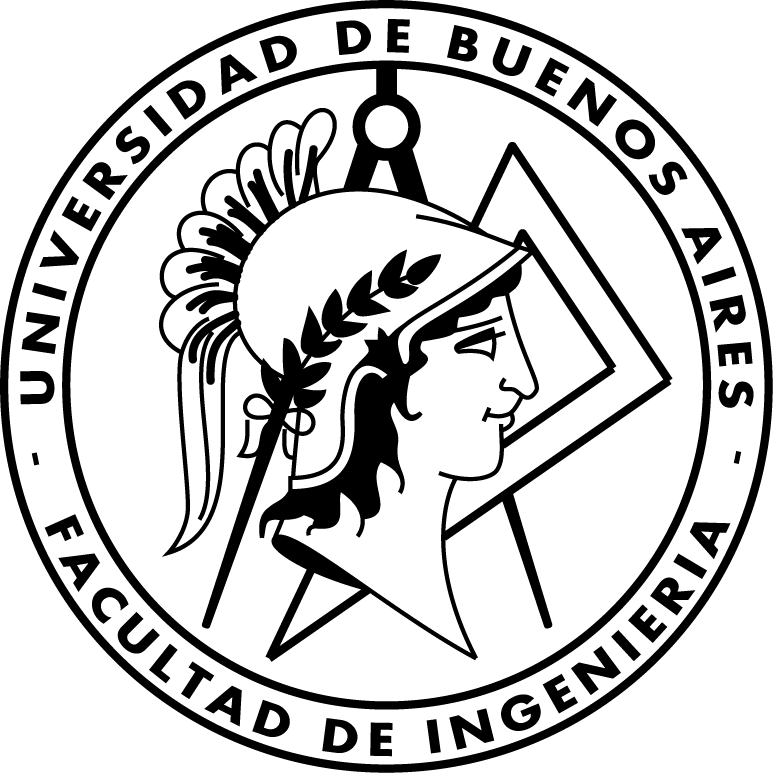
\includegraphics[scale=1]{../../Pictures/fiuba.png}}

\author{	Francisco Hermani, \textit{Padrón Nro. }                     \\
            \texttt{ o@gmail.com }                                              \\[2.5ex]
            Cotarelo Rodrigo, \textit{Padrón Nro. 98577}                     \\
            \texttt{ cotarelorodrigo@gmail.com }                                              \\[2.5ex]
			Agostina Vázquez, \textit{Padrón Nro. }                    
\\
            \texttt{ @gmail.com }                                              \\[2.5ex]
            \normalsize{1er. Cuatrimestre de 2019}                                      \\
            \normalsize{95.02 Base de Datos}  \\
            \normalsize{Facultad de Ingeniería, Universidad de Buenos Aires}            \\
       }
\date{26/06/2019}


\begin{document}

\maketitle
\thispagestyle{empty}   % quita el número en la primer página
\newpage

\section{Parser de los archivos HTML provistos por la cátedra}
Este punto fue implementado exclusivamente en el notebook html scrapper, con el objetivo principal de interpretar y parsear los archivos HTML que nos proporcionó la cátedra para obtener una información preliminar de los vuelos.Así, logramos generar una serie de archivos pkl con los siguientes atributos de cada vuelo: aerolínea, horario de salida y de llegada, terminal de salida y de llegada, puerta de salida y de llegada, origen y destino. En puntos posteriores se verá que no todos los atributos nos resultaron de gran valor, razón por la cual algunos fueron dejados de lado.


\end{document}



